\genHeader

Welcome to Part V, an introduction to unidirectional model-to-text transformations via Triple Graph Grammars (TGGs). If you're just joining us in this part
without completing any of the previous, be aware that while we do include references to relevant parts where required, we recommend working through
Part I for the required set up and installation instructions to ensure eMoflon is working correctly, and strong encourage completing Part IV to master
of basics of TGGs. That Part will be a key reference if you're ever unsure how to complete something here.

As we've mentioned, the goal of Part V is to continue using TGGs, but in a different context. In previous parts, we created \texttt{LeitnersLearningBox}, a
fully functioning memorization tool that stored cards (with keywords on the front, and definitions on the back) in different partitions, which could then move
throughout the box based on a set of rules. This metamodel was used in Part IV as a source language in a \emph{bidirectional} TGG transformation, where
each card was translated into an entry (with a sole content attribute storing all of a card's information) into a single dictionary container. In this part,
instead of transforming elements from one instance model into another, we want to perform a \emph{unidirectional} transformation from a textual instance of a
model into a \texttt{Dictionary}. We'll use a popular \texttt{ANTLR} parser and unparser, then define a set of rules to handle the information using eMolfon's
standard \texttt{MocaTree} language.

When establishing a model-driven solution, \emph{model transformations}\define{Model~Transformation} usually play a central and important role. This could be
for specifying dynamic semantics (as done with our learning box) or, more generally, for transforming a certain model to another model to achieve some goal
(i.e., consistency, adding or abstracting from platform details, \ldots).

There are many \emph{types} of model transformations and \cite{CH03,Mens_Gorp_2006} give a nice and detailed classification along a set of different
dimensions.\define{Model-to-~Text~Trans\-form\-ations} In this chapter, we shall explore some of these dimensions and learn how \emph{model-to-text}
transformations can be achieved with a nice mixture of \emph{string grammars} and \emph{graph grammars}.

For the rest of the chapter a model transformation is to be denoted as:
\begin{displaymath}
 	\Delta: m_{src} \rightarrow m_{trg}
\end{displaymath}
where the source model $m_{src}$ is to be transformed to the target model $m_{trg}$. Let's review the four primary ways in which $\Delta$ can be classified.

$\Delta$ is \emph{endogenous}\define{Endogenous}, if $m_{src}$ and $m_{trg}$ conform to the same metamodel. Each story driven model (SDM) built in Part III for
\texttt{LeitnersLearningBox} are examples of \emph{endogenous} transformations.

$\Delta$ is \emph{exogenous}\define{Exogenous}, if $m_{src}$ and $m_{trg}$ are instances of different metamodels. For example: A dictionary is used to learn new
words (similar to a learning box), but is more suitable for use as a reference (i.e., one already knows the words, but may occasionally need a specific
definition). In contrast, a learning box is geared towards the actual memorization process. Therefore, once could start with a learning box and, once all the
words have been memorized, transform it into a personalised dictionary for future reference. It too many words become forgotten, the dictionary should be
transformed \emph{back} to a learning box. The learning box to dictionary transformation and vice-versa are therefore examples of \emph{exogenous}
transformations, and we will create this by complementing our \texttt{LeitnersLearningBox} with a simple language for \texttt{Dictionary}.

$\Delta$ operates \emph{in-place}\define{In-place Model~Trans\-form\-ation} if $m_{src}$ is \emph{destructively} transformed to $m_{trg}$. The SDMs for our
learning box (e.g. \texttt{grow} or \texttt{check}) are examples of \emph{in-place} transformations as they perform destructive changes directly to a source
model, transforming it into the target model.

Finally, $\Delta$ is \emph{out-place}\define{Out-place Model~Trans\-form\-ation} if $m_{src}$ is left intact and is unchanged by the transformation which
creates $m_{trg}$. The learning box to dictionary transformation and vice-versa (that we will implement in this part) are examples of \emph{out-place}
transformations.

Although \emph{endogenous} + \emph{in-place} is the natural case for SDMs (as was the case for our learning box), \emph{exogenous} and/or \emph{out-place}
transformations can still be specified. Using the basics introduced in Part IV: Triple Graph Grammars however, we will implement this latter type with
TGGs.
 
\newpage
 
To twist your brain a bit, here are a few interesting statements:
\begin{enumerate}

\item[$\blacktriangleright$] \emph{Out-place} transformations can be \emph{endogenous} or \emph{exogenous}.

\item[$\blacktriangleright$] \emph{In-place} transformations can usually only be \emph{endogenous}. \emph{Exo\-gen\-ous} transformations are consequently,
always \emph{out-place}.  Why?

\end{enumerate}  

It should be noted that $\Delta$ \define{Abstraction Levels}can be further classified as \emph{horizontal} if $m_{src}$ and $m_{trg}$ are on the same
\emph{abstraction level}, or \emph{vertical} if they are not. Unfortunately, this \emph{abstraction level} dimension is a bit `fuzzy,' but we will explore and
work on these different levels by establishing a textual concrete syntax for \texttt{Dictionary}. We shall learn how graph transformations can be used in
combination with parser generators and template languages to implement model-to-text and text-to-model transformations that are typically \emph{vertical} (text
is normally on a lower abstraction level than a model). On the other hand, the overall learning box to dictionary transformation is \emph{horizontal} as the
models represent the \emph{same} information differently, and can thus be considered to be on the same abstraction level.

In the following, the \emph{\bf Mo}flon \emph{\bf C}ode \emph{\bf A}dapter (\emph{Moca}) framework refers to:
\begin{enumerate}

 \item The approach we use to integrate string grammars, graph grammars and template languages, 

 \item how we separate the transformation into different modular steps, 

 \item the use of a generic and simple tree to consolidate different platforms, and 

 \item the actual tool support that acts as glue to hold all the different parts together.

\end{enumerate}

% Fig.~\ref{fig:moca-overview} gives a ``big picture'' of what we plan to achieve in this part of the eMoflon handbook. All explanations are integrated right with
% the figure, so take your time to read it carefully and let it sink in. We'll be zooming in the bits and pieces of each step in the following sections to clear
% up any confusion.

% \begin{figure}[htp]
% \begin{center}
%  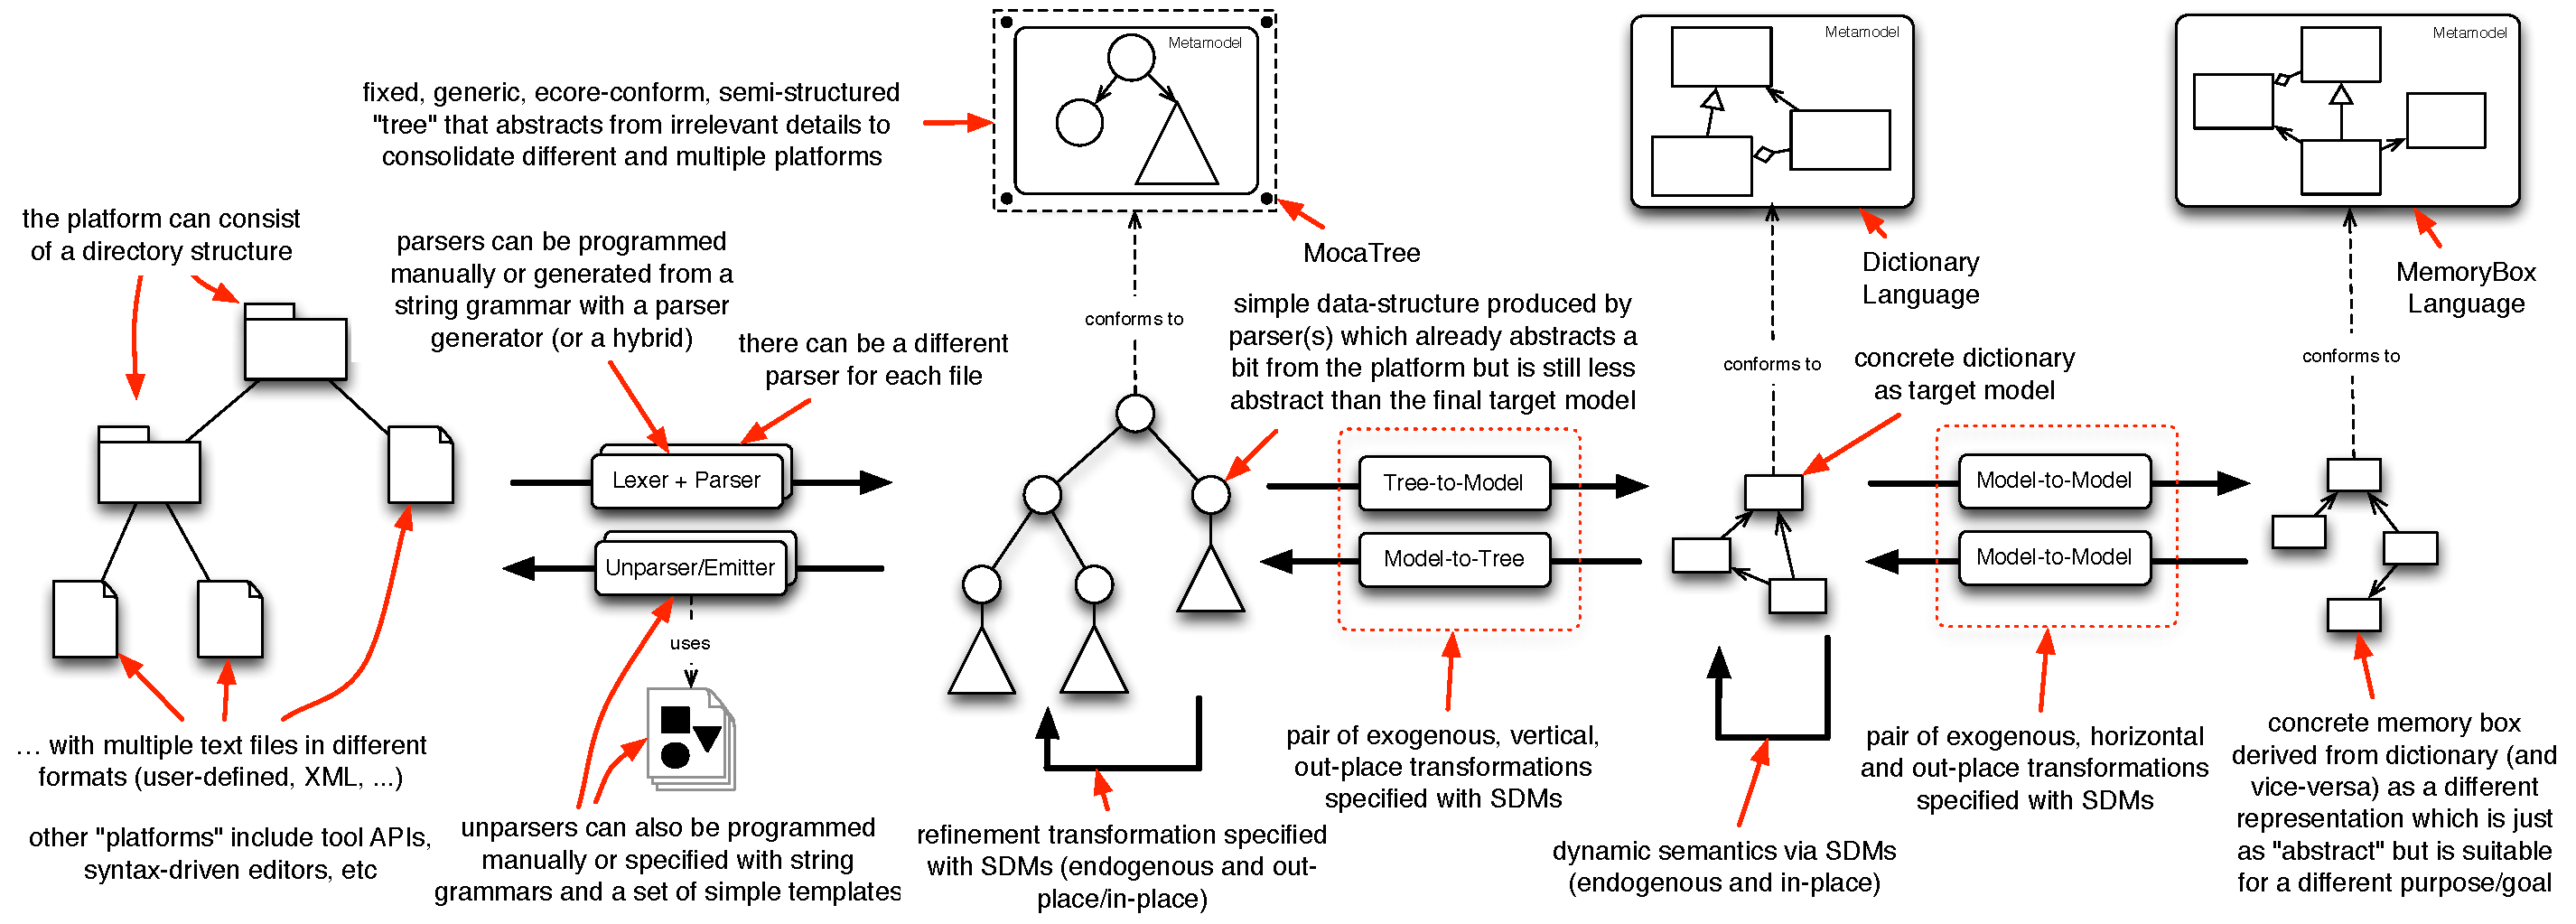
\includegraphics[angle=90, height=\textheight]{pics/moca/text-to-model}
%   \caption{Overview of model-to-text with the MOCA framework}
%   \label{fig:moca-overview}
% \end{center}
% \end{figure} 

Before starting, let's quickly summarise the transformation we hope to complete. We want to be able to take a generic filesystem containing some plain text
files and translate them into a new model. Not only will this require the contents of those files be to formatted a certain way so they may be parsed, the
transformation will not be able to go directly from the files to a instance model. Instead, it will need to be read to and from a tree structure. Thus, our forward and backwards transformations will each
be broken into two steps: text-to-tree, tree-to-model, and vice versa.
